\section{接回回路：能力、反馈与承责的位置}

三层塌陷可以互相强化。专业位置削弱，使即时认可更有吸引力；很少检验判断的反馈环境，减少了校准的练习；信心下降、替代路径变少，又让人更难回到有效位置。每一条连接都可以调查，每一条连接也都可能成为干预点。

\subsection{三只时钟与几条修复路径}

职业结构可能按年变化，界面可以按周调整，技能、习惯与关系则各有形成周期。成年后的学习与恢复仍然持续。干预需要找准对应过程，及时保住仍可改善的部分。

把进入一种替代体验的成本记为$c_n$，可以写出一个简化递推：
\begin{equation}
c_{n+1}=Gc_n,\qquad G=g_1g_2g_3.
\end{equation}
若三个正乘数都小于1，模型中的进入成本便逐圈下降。这个式子只描述所定义的成本。完整社会回路还需要职业位置、反馈与主体性的独立状态变量，以及延迟、外部输入和可观察的因果连接。

\begin{figure}[ht]
\centering
% >>>>>>>>>> figs/fig-collapse-cycle.tex >>>>>>>>>>
% 图 5-3  三级下沉的回路结构
% (a) 三节点回路：功能层 → 真实层 → 主体层 → 功能层，三条弧上各带一个削减比例
%     $g_i$，环心给出传递关系。节点第二个小字是各层的时间尺度。
%     $g_i=1$ 表示该层不再以更低的门槛把代价传给下一层。
% (b) 门槛 $c_n$ 随圈数的下降：$c_n=G^n$，对数纵轴。三条线对应 G=0.5 / 0.8 / 1.0，
%     说明「取消一节只是放慢、三节都取消才停住」。
% 与图 5.1 的分工：那张画的是三层之间的**链**（谁把谁推向哪里），
% 这张画的是那条链首尾相接之后的**回路**与其传递系数，正文明确区分过这两者。
%
% 版心宽 144mm，这张图按 \useasboundingbox 算到 138mm——第一版画到 149mm，
% 编译时在 \end{tikzpicture} 处报 14.2pt overfull。盒子从 2.60 收到 2.30、
% (b) 的横轴从 0.58/格 收到 0.50/格之后才装得下。改之前先量总宽。
\begin{tikzpicture}[x=1cm, y=1cm, font=\small,
  bn/.style={draw, line width=0.7pt, rounded corners=2pt,
             minimum width=2.30cm, minimum height=0.94cm, align=center,
             inner sep=2pt, text=ink},
  gl/.style={font=\small, text=ink, inner sep=1pt},
  ax/.style={-{Stealth[length=2.0mm]}, ink, line width=0.6pt},
  tick/.style={font=\scriptsize, text=slate}
]
\useasboundingbox (-0.85,-0.50) rectangle (12.95,-7.30);

% ================= (a) 三节点回路 =================
\node[bn, draw=terra!60, fill=terra!13] (f) at (3.30,-1.30)
      {功能层\\[0.5pt]{\scriptsize\color{slate}年}};
\node[bn, draw=rust!60,  fill=rust!13]  (r) at (6.10,-5.70)
      {真实层\\[0.5pt]{\scriptsize\color{slate}月—年}};
\node[bn, draw=forest!60, fill=forest!13] (s) at (0.50,-5.70)
      {主体层\\[0.5pt]{\scriptsize\color{slate}代}};

% 顺时针三边：功能层→真实层→主体层→功能层
\draw[-{Stealth[length=2.2mm]}, slate!70, line width=0.9pt] (f) -- (r);
\draw[-{Stealth[length=2.2mm]}, slate!70, line width=0.9pt] (r) -- (s);
\draw[-{Stealth[length=2.2mm]}, slate!70, line width=0.9pt] (s) -- (f);

% 环心的传递关系。分两行写：单行放不进三角形内空（内空最窄处约 3.4cm）。
\node[font=\small, text=ink] at (3.30,-3.95) {$c_{n+1}=G\,c_n$};
\node[font=\small, text=ink] at (3.30,-4.34) {$G=g_1g_2g_3<1$};

% 三个削减比例，放在各边外侧（沿外法向偏移 0.45cm，已核对仍在三角形之外）
\node[gl] at (5.08,-3.26) {$g_1$};
\node[gl] at (3.30,-6.22) {$g_2$};
\node[gl] at (1.52,-3.26) {$g_3$};

% ================= (b) 门槛随圈数下降 =================
% \bx 不能再小：纵轴刻度字「0.01」以轴心右对齐，左端伸到轴外约 0.75cm，
% 8.45 时它的左端在 7.62，正好让开真实层盒子的右缘 7.25。
\def\bx{8.45} \def\bdx{0.50} \def\byB{-6.16} \def\bah{4.20}
\def\yy#1{\byB+\bah*(log10(#1)+2)/2}   % c=1 在上端，c=0.01 在下端，两个数量级

\draw[ax] (\bx,\byB) -- ({\bx+\bdx*6+0.42},\byB)
      node[anchor=west, font=\scriptsize, text=ink] {$n$};
\draw[ax] (\bx,\byB) -- (\bx,{\byB+\bah+0.30})
      node[anchor=south, font=\scriptsize, text=ink] {$c_n$};

% 纵轴刻度：1 / 0.1 / 0.01。只标这三条，其余留给曲线。
\foreach \c in {1,0.1,0.01} {
  \draw[slate!55, line width=0.45pt] ({\bx-0.07},{\yy{\c}}) -- ({\bx+0.07},{\yy{\c}});
  \node[tick, anchor=east] at ({\bx-0.13},{\yy{\c}}) {\c};
}
% 横轴刻度：圈数 0--6
\foreach \k in {0,...,6} {
  \draw[slate!55, line width=0.45pt] ({\bx+\bdx*\k},{\byB-0.07}) -- ({\bx+\bdx*\k},{\byB+0.07});
  \node[tick, anchor=north] at ({\bx+\bdx*\k},{\byB-0.12}) {\k};
}

% 三条 c_n=G^n。G 越大下降越慢，G=1 是一条水平线。
% 先画陡的，最后画平的，免得被压在下面。
\foreach \G/\cl in {0.50/rust, 0.80/terra, 1.00/forest} {
  \draw[\cl, line width=1.3pt]
    \foreach \k in {0,...,5} {
      ({\bx+\bdx*\k},{\yy{pow(\G,\k)}})
      -- ({\bx+\bdx*(\k+1)},{\yy{pow(\G,\k+1)}})
    };
}

% 曲线右端的标签。纵坐标由同一式子算出，不手填，免得改了曲线忘了改标签。
\pgfmathsetmacro\yA{\yy{1.0}}
\pgfmathsetmacro\yB{\yy{0.8^6}}
\pgfmathsetmacro\yC{\yy{0.5^6}}
\node[anchor=west, font=\scriptsize, text=forest] at ({\bx+\bdx*6+0.14},\yA) {$G=1$};
\node[anchor=west, font=\scriptsize, text=terra]  at ({\bx+\bdx*6+0.14},\yB) {$G=0.8$};
\node[anchor=west, font=\scriptsize, text=rust]   at ({\bx+\bdx*6+0.14},\yC) {$G=0.5$};

% ================= 栏标题（一律在内容下方）=================
\node[anchor=north, font=\footnotesize\heiti, text=slate] at (3.30,-6.72) {(a) 三层的回路};
\node[anchor=north, font=\footnotesize\heiti, text=slate] at (9.95,-6.72) {(b) 门槛的逐圈下降};
\end{tikzpicture}

% <<<<<<<<<< figs/fig-collapse-cycle.tex <<<<<<<<<<

\caption{进入成本的简化递推。假设三个正成本乘数固定且均小于1，乘积决定成本曲线的下降速度。图示说明这个成本模型，不代表职业、反馈与主体性的完整因果动力学；真实干预还可改变乘数、结构与外部输入。}
\label{fig:collapse-cycle}
\end{figure}

调查可以先从较窄的问题开始：进入一项职业是否更难？辅助工具改善了独立测试的技能，还是只提高即时产出？使用者能否识别、质疑并纠正一次重要错误？申诉是否改变决定？替代路径是否负担得起、实际可用？

这些问题需要不同证据：纵向观察、任务测试、机构记录与具体案例。指标还要接受反向检查，避免把“记录了多少次申诉”误当成“解决了多少问题”。恢复机制需要有实际改变过程的能力。

\subsection{承责结构的四项功能}

后果需要一条进入回应的路径。承责结构至少要提供四项功能。

\textbf{发现。}监测损害、险情与重要偏离；让使用者和受影响者能够报告问题。运营方的仪表盘与外部投诉入口要能够相接。

\textbf{追溯。}把事件接回相关决定、版本、配置与工具行动。记录的范围、保存期限、访问权限与隐私保护，需要随用途一起设计。

\textbf{止损。}让某个位置拥有实际可用的暂停、隔离、召回或限制权。紧急控制可以先于完整归因，避免调查期间继续扩大损害。

\textbf{救济。}让受影响者能够要求纠错、获得适当补偿，并推动防止复发。责任背后的资产、保险与组织能力，决定了承诺能兑现多少。

\begin{figure}[ht]
\centering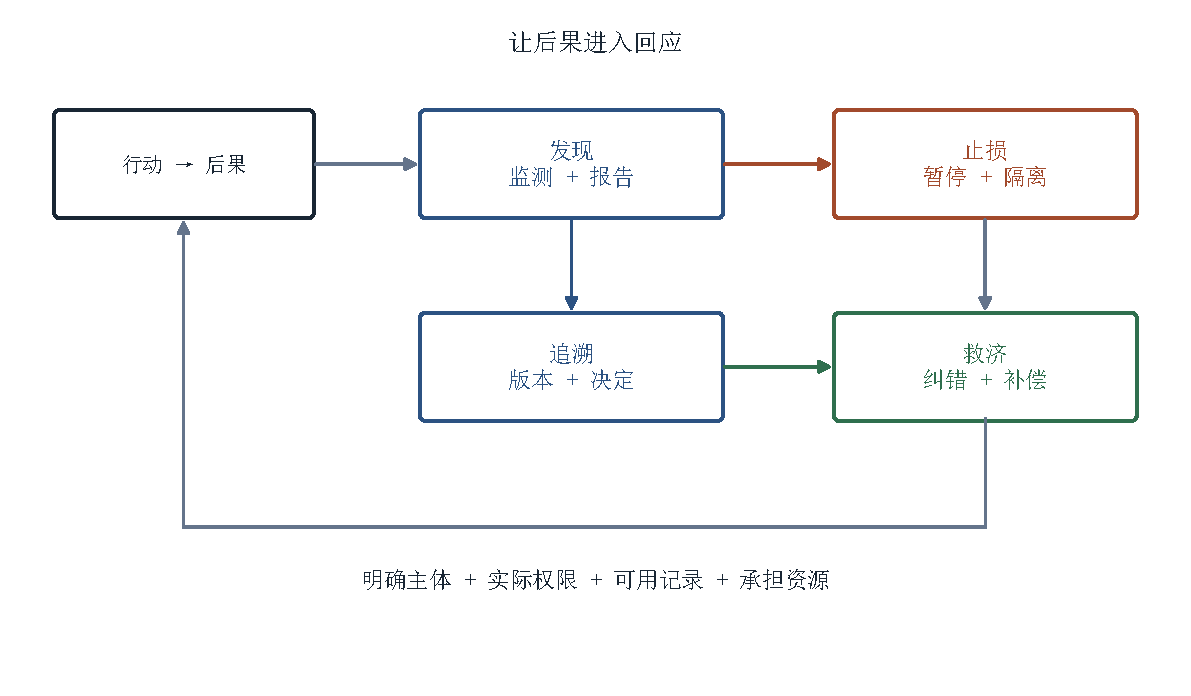
\includegraphics[width=\textwidth]{figures/accountability.pdf}
\caption{承责的四项功能。监测和报告使后果进入记录，追溯提供解释与纠错依据；止损可以立即启动，救济继续处理已发生的后果。四项功能相互连接，并可并行运行。}
\label{fig:accountability-loop}
\end{figure}

四项功能可以并行，也会互相提供输入。每一项都需要主体、资源与操作接口。航空业把设计保证、生产控制、维护、运行权限、报告与调查组织在一起，可靠性由航空器和制度共同形成。其他领域也需要根据自己的后果与控制条件安排这些功能。

机器系统的接口需要同样清楚：谁控制更新，谁能暂停访问，服务停运后哪些记录仍在，谁受理对模型决定的异议，谁有能力承担救济？

责任可以依据控制能力、合同角色、法定义务与其他正当标准分配。保险与补偿基金能够分担部分损失，独立调查有助于把学习与即时归责区分开。激励、执行和资金共同决定这些安排是否真正工作。

承责也能扩大部署。风险具有明确控制、记录和救济路径，就更容易被评估和采用。系统知道不确定性变成后果时如何行动，一部分原本难以承诺的应用才获得可运行条件。

\subsection{判断需要资格}

三个问题始终留在决定的核心：哪些后果可以接受，多少证据足以行动，谁有权把代价施加给谁。

模型可以估计结果、比较方案、揭示矛盾，也能帮助人表达立场。采用标准与施加后果，还需要相应权利、授权和职责。本书主张：\key{承担后果的人，应当保有有效发言、代表与质疑的渠道。}

直接暴露构成一种资格来源；合法委托、专业义务、民主授权，以及对缺席者和弱势者的保护，也构成资格来源。患者承担身体风险，医师承担专业责任，两种位置通过知情同意、专业标准与追责程序连接起来。陪审员通常不承受被告同样的后果，其权限来自法律赋予的角色、义务与程序。\cite{kalven1966american}

机长、医师、陪审员各有不同依据。共同要求是：决定有可说明的理由，权限有明确范围，受到质疑时有人必须回应。复核者还要具备能力、时间和改变决定的权力，纸面的“人在回路”才会成为实际位置。

\subsection{产出变便宜，人的价值如何成立}

只按稀缺产出衡量人的社会，会在产出变丰裕时失去一部分价值尺度。参与、照护、关系、判断与有限生命，需要进入更完整的评价。

后果落在某个人身上，使这个人获得保护与发言的理由。负担如何分配，还要依照正当的权力和控制关系来判断。承担本身无须被浪漫化，能够减少的伤害应当减少。

另一个人可以提供建议、劳动或受托决定，却不能因此替你活完同一段有限生命，也不能自动占据同一关系。辅助扩大一个人的能力，这个人在结果中的利害仍然存在。

修复的方向因此很具体：重建进入有用贡献的路径，保留能够纠错的反馈，让退出、异议和长期承诺继续可行，把有后果的行动接回能够回应的人与机构。它们需要投入。下一章继续区分：哪些成本只是在阻挡，哪些成本维护了进步值得拥有的条件。

\furtherreading{%
Hannah Arendt，\textit{The Origins of Totalitarianism}\\
Herbert Marcuse，\textit{One-Dimensional Man}\\
Jean Baudrillard，\textit{Simulacra and Simulation}\\
René Girard，\textit{Deceit, Desire, and the Novel}\\
Harry Kalven Jr.\ \& Hans Zeisel，\textit{The American Jury}\\
Ivan Illich，\textit{Tools for Conviviality}\\
Cathy O’Neil，\textit{Weapons of Math Destruction}\\
Theodore Kaczynski，\textit{Industrial Society and Its Future}}


% <<<<<<<<<< parts/book-ch05.tex <<<<<<<<<<


% >>>>>>>>>> parts/book-ch06.tex >>>>>>>>>>
%% ===================== 本章参考文献 =====================
\printbibliography[heading=subbibliography,title=参考文献]
